\documentclass[a4paper, 12pt]{article}
\usepackage[utf8]{inputenc}
\usepackage[francais]{babel}
\usepackage[pdftex]{graphicx}
\usepackage{hyperref}
\usepackage{titlesec}

\titleformat*{\section}{\LARGE\bfseries}
\titleformat*{\subsection}{\large\bfseries}

\begin{document}
\begin{titlepage}
\begin{center}

{\Large Université de Mons}\\[1ex]
{\Large Faculté des sciences}\\[1ex]
{\Large Département d'Informatique}\\[2.5cm]

\newcommand{\HRule}{\rule{\linewidth}{0.3mm}}
% Title
\HRule \\[0.3cm]
{ \LARGE \bfseries Quoridor \\[0.3cm]}
{ \LARGE \bfseries Rapport de projet \\[0.1cm]} % Commenter si pas besoin
\HRule \\[1.5cm]

% Author and supervisor
\begin{minipage}[t]{0.45\textwidth}
\begin{flushleft} \large
\emph{Professeur:}\\
Hadrien \textsc{Mélot}\\
\end{flushleft}
\end{minipage}
\begin{minipage}[t]{0.45\textwidth}
\begin{flushright} \large
\emph{Auteurs:} \\
Virgil \textsc{Surin} \\
Simon \textsc{Michel}
\end{flushright}
\end{minipage}\\[2ex]

\vfill

% Bottom of the page
\begin{center}
\begin{tabular}[t]{c c c}

\includegraphics[height=1.5cm]{logoumons.jpg} &
\hspace{0.3cm} &

\includegraphics[height=1.5cm]{logofs.jpg}
\end{tabular}
\end{center}~\\
 
{\large Année académique 2019-2020}

\end{center}
\end{titlepage}

\tableofcontents

\newpage

\section{Introduction}

Ce projet à pour objectif de ré-implémenter en Java le jeu de plateau Quoridor mais également de nous permettre d'apprendre à développer de A à Z une application fonctionnelle relativement importante en terme de taille et de complexité (pour notre niveau de première année du moins). \\

Ce projet est également l'occasion pour nous d'apprendre à nous organiser, à travailler en groupe mais également d'apprendre à chercher par nous même des solutions à des problèmes. \\

Afin de le mener à bien il nous a fallu du temps, beaucoup de réflexion mais aussi beaucoup de tests et d'essais. Nous avons crée plusieurs prototypes afin d'expérimenter des concepts, peser les pours et les contres pour au final arriver au résultat que vous avez sous vos yeux.

\section{Mode d'emploi}

Le jeu mode graphique du jeu se lance avec la commande \textit{gradle run} précédée d'un
\textit{gradle build}. Le menu se lance alors, vous pouvez choisir les paramètres de la
partie ou en charger une si une partie a déjà été sauvegardée. \\

Afin de déplacer votre pion, vous devez faire un clique gauche sur celui-ci, les différents déplacements possibles seront mis en évidence. En deuxième clique gauche sur la case souhaitée vous y déplacera. \\

Afin de placer des murs, maintenez le clique droit de la souris pour faire apparaître un mur fantôme. Placez le mur fantôme à l'endroit désiré et faites un clique gauche pour le placer. Si le mur disparait c'est qu'il bloquait un joueur.
Un clique gauche ailleurs que sur la case où se trouve le mur le fera disparaitre. \\

Vous pouvez à tout moment appuyer sur la touche \textit{ECHAP} du clavier pour faire apparaître le menu pause qui vous permet de sauvegarder ou de retourner au menu principal.

\section{Répartition des tâches}
\begin{itemize}
\item[•] Conception du modèle : Simon MICHEL et Virgil SURIN
\item[•] AI : Simon MICHEL
\item[•] Logique de jeu : Virgil SURIN
\item[•] Interface utilisateu : Simon MICHEL et Virgil SURIN
\item[•] Traduction du modèle en Java :Virgil SURIN
\item[•] Création des sprites : Simon MICHEL
\item[•] Système de sauvegarde : Simon MICHEL
\item[•] Test unitaires : Virgil SURIN
\end{itemize}

\section{Choix personnel}

\subsection{Règle spéciale pour 4 joueurs}
Nous voulions implémenter le mode 4 joueurs et, à l'origine, suivre les règles officielles du jeu. Mais il nous est apparu qu'elles avaient une faille. En effet il n'est possible, dans les règles officielles, de sauter que par dessus un seul pion :
\begin{center}
\includegraphics[scale=0.3]{regle-officiel.png} \\
\textit{Règle officielle.}
\end{center}

Mais il existe un cas où un joueur peut se retrouver sans mur et sans possibilité de se déplacer à cause d'autres pions :
\begin{center}
\includegraphics[scale=0.3]{rp.png} \\
\textit{Si le joueur bleu n'a plus de mur et que les deux autres oui, ils peuvent poser des murs pour passer les tours et le joueur bleu ne peut alors rien faire.}
\end{center}
Nous avons donc décidé d'autoriser les joueurs à sauter par-dessus plusieurs pion comme suit si les déplacements sur le côtés ne sont pas possibles :
\begin{center}
\includegraphics[scale=0.3]{r2.png} \\
\textit{Le joueur bleu peut sauter tout les autres pions.} \\
\includegraphics[scale=0.3]{r1.png}
\includegraphics[scale=0.3]{r3.png} \\
\textit{Si le joueur bleu rencontre un mur alors il regarde sur les côtés pour effectuer son déplacement.} \\
\includegraphics[scale=0.3]{r4.png} \\
\textit{Si le joueur peut aller sur le côté alors il le fait.}
\end{center}



Cela règle le soucis du joueur bloqué lors de partie  à 4 joueurs. 


\subsection{Le plateau et les murs}
Le premier choix que nous avons fait est certainement la façon dont nous allions gérer le plateau et les éléments qui allaient le composer et surtout comment s'occuper correctement
des murs. \\

Tout d'abord, nous avons fixé un système de coordonnée (y,x) où la case la plus en haut à gauche sera l'origine (0,0) et celle en bas à droite aura la coordonnée (t-1,t-1) où \textit{t} représente la taille du plateau (qui sera toujours carré). \\

Pour le murs, nous avons réfléchis et deux approches se sont présentées : 
\begin{itemize}
\item[•] Créer une grille avec des cases pions et des cases murs
\item[•] Ne faire qu'une grille pour pions et donner aux cases la possibilité de savoir sur quel côté il y un mur.
\end{itemize}
Nous avons choisi après longue réflexion la deuxième solution. Elle nous semblaient plus simple car elle ne nécessitait pas de créer plusieurs types de cases différentes. De plus, cette solution demande uniquement une grille simple qui représente le plateau et il nous semblait aussi plus simple d'interroger la case pour savoir si elle possède un mur dans une direction donnée que de chercher dans une grille parallèle. Également, le déplacement nous semblait plus naturel à implémenter : \\
\textit{e.g :} pour faire un déplacement vers la droite il suffit d'ajouter 1 en abscisse. \\

Pour placer les murs sur le plateau, étant donné que nous n'avions pas de grille spéciale pour ça, nous avons adopté la convention suivante : \\
\begin{itemize}
\item[•] un mur se pose uniquement sur le côté droit ou le côté supérieur d'une case.
\item[•] un mur posé sur le côté droit sera vertical et ira vers le haut.
\item[•] un mur posé sur le côté supérieur sera horizontal et ira vers la droite.
\end{itemize}
\begin{center}
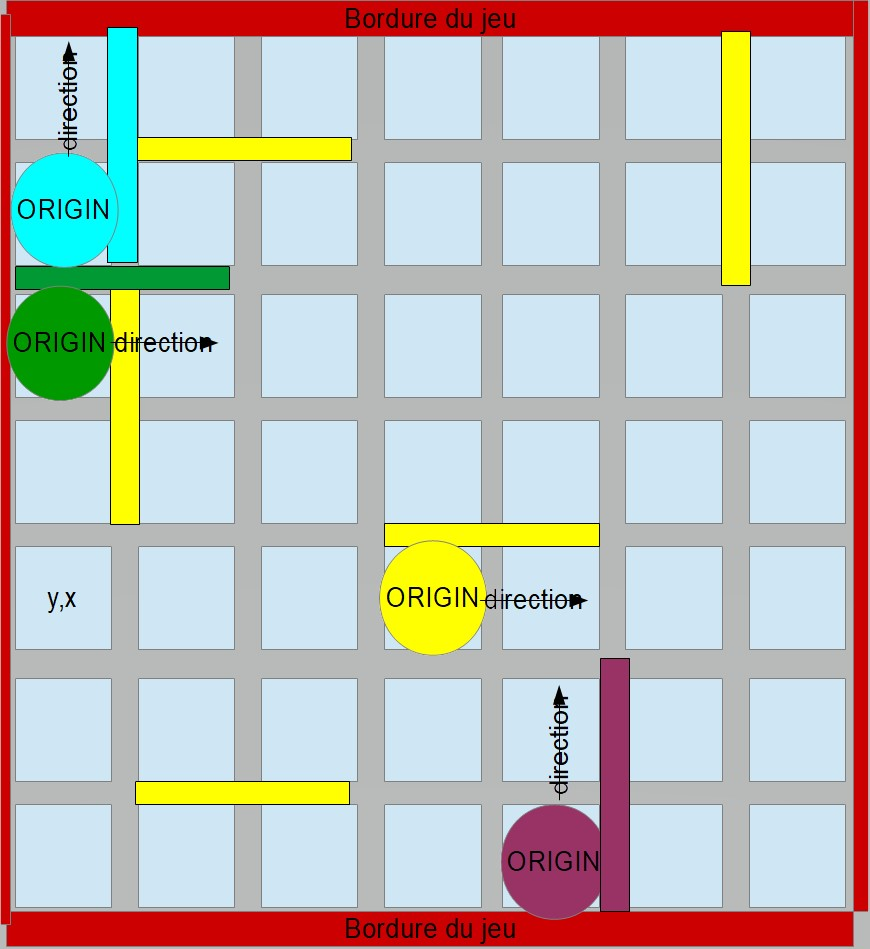
\includegraphics[scale=0.3]{wall.jpg} \\
\textit{Illustration du placement des murs.}
\end{center}
Avec cette convention, nous sommes sûr de pouvoir poser tout les murs possibles et imaginables. De plus, elle nous donne des hypothèses utiles pour l'implémentation des règles. Les murs étant stocké par le plateau dans une liste dont chaque élément est un tableau composé de la coordonnée d'origine du mur et de celle de la deuxième case à laquelle il est attaché, on peut grâce à ça facilement déterminer si c'est un mur vertical ou horizontal. On peut également aisément voir grâce à se format si deux cases adjacentes ont un mur continu sur leur côté ou non. Pour le savoir il suffit de regarder dans la liste des murs s'il existe un tableau composé de d'abord la coordonnée de la case avec le plus petit abscisse ou la plus grande ordonnée suivi en dernière position de la coordonnée de l'autre case.

\subsection{Structure du modèle}
Une chose qu'il a fallu clarifier tôt dans le développement est la structure du modèle.
Nous avons décider d'opter pour un objet \textit{Game} qui allait contenir touts les éléments de la partie en cours. Ce qu'il nous faut pour le jeu de base, c'est un plateau, des pions et des murs. Mais dans un but de modularité et pour pouvoir dans le futur rajouter des fonctionnalités, nous avons créer des catégories qui donneront nos packages :
\begin{itemize}
\item[•] \textit{world} : contient tout ce qui est relatif au monde dans lequel le jeu se déroule, dans notre cas c'est un simple plateau et des cases.
\item[•] \textit{item} : contient tout les éléments du jeu, toutes les pièces comme les pions et les murs mais pourquoi pas des outils ou des power-up dans le futur ?
\item[•] \textit{controller} : contient les entités chargées de contrôler les \textit{items}, par exemple, un PawnController est conçu pour pouvoir contrôler un pion et rien d'autre.
\item[•] \textit{engine} : contient tout ce qui est relatif à la logique de jeu ou le bon fonctionnement de celui-ci comme les règles mais aussi le jeu lui-même, les différentes IA et le système de sauvegarde.
\item[•] \textit{tool} : ce package un peu spécial contient des outils généraux qui servent à de multiples endroits dans le projet. Pour l'instant, il ne contient que la classe de coordonnées.
\item[•] \textit{gui} : c'est ce package qui va s'occuper de toute l'interface utilisateur mais aussi de la gestion du joueur humain.
\end{itemize}
Cela c'est avéré être une base solide. Nous avons avec ça mis au point une hiérarchie simple pour \textit{item} et \textit{controller} où ces deux packages contiennent chacun une classe abstraite mère qui représente l'élément le plus basique possible dans sa catégorie. Chaque autre classes héritent de leur classe mère afin de s'assurer que chacun ai le minimum syndicale pour être dans le jeu.

\subsection{Le pathfinding}
Tout les chemins mènent à Rome mais aussi tout les moyens de transports ! Il a donc fallu choisir entre les différentes façon de trouver le chemin le plus courts. \\

Dans sa thèse \textit{Mastering Quoridor}, Lisa GLENDENNING explique qu'elle a choisi de voir le plateau comme un graphe et utilise donc \href{https://en.wikipedia.org/wiki/Dijkstra_algorithm}{l'algorithme de Dijkstra}. Nous avons donc envisagée cette option mais bien qu'efficace elle nous semblait trop difficile à implémenter. Nous avons finalement opté pour l'algorithme présenté en séance par les assistants : le \href{https://en.wikipedia.org/wiki/Breadth-first_search}{breadth-first search} \textit{i.e} le parcours en largeur.

\subsection{Le placement des murs par l'utilisateur}
Etant donné notre système de gestion des murs, il n'était pas réellement possible de se baser sur les interstices entre les cases pour placer les murs. Nous avons donc décidé de coller à notre modèle et de découper chaque case en deux. Un mur se pose sur une case et selon la position de la souris sur cette case, on lui donne une direction. La moitié supérieur de la case donne un mur horizontal et la partie inférieure donne un mur vertical. \\
Nous avons conscience que ce système est moins intuitifs. Cela montre donc la raison pour laquelle le jeu en ligne est implémenté avec l'autre système qui nous avions envisagé.

\subsection{La résolution}
Nous avons décider de mettre la résolution de base de notre jeu à 700x700. Bien entendu, l'utilisateur peut redimensionner à sa guise la taille de la fenêtre. Lorsqu'une partie est lancée, la fenêtre se redimensionne à la taille que nous avons jugée minimale afin de voir l'ensemble du plateau. \\

Pourquoi ce choix de 700x700 ?  Bien que la grande majorité des écrans actuels soient en 1920x1080, il ne faut pas négliger les autres formats et écrans plus vieux. Cette résolution de 700x700 nous a semblé être une taille suffisante que pour être affichée correctement sur tout les écrans ou presque.

\section{Algorithme}

\subsection{Le pathfinding}
Comme dis précédemment, nous avons choisis d'implémenter le \textit{breadth-first search}. \\

L'idée est donc de partir du pion et d'explorer toute les cases possible aux alentours. Ensuite, toutes ses cases nouvellement explorées doivent être explorées à leur tour et ainsi de suite jusqu'à ce qu'on ai trouvé un case qui rempli la condition de victoire. Etant donnée que chaque case renvoie vers la case depuis laquelle on l'a explorée, on peut ensuite remonté jusqu'au pion et nous avons notre chemin le plus court. \\

Pour implémenter ceci il a fallu d'abord définir une liste de cases que l'on a déjà explorée et une liste contenant les cases qui doivent être explorées à la prochaine itération. \\

L'algorithme principal (\textit{findAPath}) initialise les différentes listes ainsi qu'une HashTable qui va contenir les liens entre les cases. Dans cette table, la clé est une case et la valeur associé renvoie vers la case dont on est venu. La case de départ est marquée avec une coordonnée spéciale, de même pour la case d'arrivée. L'algorithme va ensuite lancer des itérations (\textit{explore}) pour explorer les cases aux alentours en vérifiant qu'on explore pas deux fois la même case et qu'on respecte bien les règles de déplacement. Si \textit{explore} retourne 1 alors cela signifie qu'un chemin à été trouvé. Si il retourne 0, on continue d'itérer, si il retoure 2 alors il n'y a pas de chemin car il ne reste plus de case à explorer et dans ce cas on retourne une HashTable spéciale avec une clé particulière qui indique qu'il n'y a pas de chemin.\\

Pour traduire la HashTable en un chemin, il suffit de partir de la clé spéciale qui marque l'arrivée, et de remonter de clé en valeur à la marque de départ.

\subsection{Les règles}
Les règles n'ont pas toute été simples à implémenter. Autant la validité d'un déplacement ne demande que de vérifier si la case où l'on se trouve possède un mur dans la direction donnée autant tester la validité d'un mur est autrement plus complexe. \\

Je cite la règle officielle quant au placement des murs : \\
\textit{"La pose des barrières a pour but de se créer son propre chemin ou de ralentir l’adversaire, mais il est interdit de lui fermer totalement l’accès à sa ligne de but: il faut toujours lui laisser une solution."} \\

Cela implique de vérifier lorsqu'on souhaite placer un mur qu'il existe encore un chemin pour chaque joueur en jeux. Pour vérifier cette règle, nous copions le plateau (qui contient également les murs et les pions), nous plaçons le mur voulu et pour chaque pions nous appliquons le pathfinding. Si celui-ci ne trouve pas de chemin alors on ne peux pas placer le mur en question.\\
Ceci dit une autre vérification doit être faite : \\

On ne doit pas chevaucher et/ou couper un mur existant et/ou poser un mur en partie ou totalement hors du plateau.
Grâce à la convention prise, nous pouvons aisément empêcher les murs de sortir. En effet il suffit d'empêcher de poser des murs attachés aux cases d'ordonnée 0 et celles d'abscisse t-1. Pour éviter tout chevauchement voici la méthode utilisée.\\
\textbf{Premier cas :} \\

 Soit notre mur représenté par [(y, x1),(y, x2)]\footnote{rappel : x1 = x2-1} il y a chevauchement dans les cas où les murs suivant existent dans la liste des murs du plateau :
\begin{itemize}
\item[•] [(y, x1),(y, x2)]
\item[•] [(y, x1-1),(y, x1)]
\item[•] [(y, x2),(y, x2+1)]
\end{itemize}
\textbf{Deuxième cas :} \\
 Soit notre mur représenté par [(y1, x),(y2, x)]\footnote{rappel : y2 = y1-1} il y a chevauchement dans les cas où les murs suivant existent dans la liste des murs du plateau :
\begin{itemize}
\item[•] [(y1, x),(y2, x)]
\item[•] [(y1+1, x),(y1, x)]
\item[•] [(y2, x),(y2-1, x)]
\end{itemize}
Ceci fait il ne reste plus qu'à vérifier que l'on ne coupe pas un mur déjà existant : \\
Pour cela, nous devons simulé le mur qui pourrait poser problème. Pour ce faire nous prenons la direction complémentaire\footnote{Up si le mur que l'on souhaite placer va vers la droite, Right sinon}, un créer un mur dont l'origine est la même que le mur que l'on veut placer mais dont la seconde partie est donnée par l'origine + la direction supplémentaire. Il suffit ensuite de regarder si un tel mur est déjà dans la liste des murs du plateau. Si oui on ne peut placer le mur désiré. \\

Dans un soucis d'optimisation, on vérifie d'abord les collisions avec d'autres murs ou les bords du plateau avant de vérifier s'il reste encore un chemin étant donnée que la complexité du pathfinding est plus élevée que les vérifications de collision.

\subsection{Les IAs}
Lorsqu'il s'est agit de concevoir et d'implémenter les IAs, le choix le plus évident était de faire une IA entièrement aléatoire. Cette IA très facile, que nous avons affectueusement nommée "\textit{Débilus}" en coulisses, agit ainsi entièrement via l'aléatoire: elle décide aléatoirement quelle action faire entre un mouvement ou un placement de mur; si elle bouge, dans quelle direction et si elle pose un mur, où est-ce qu'elle le pose.
En toute logique, sauf par un extrême concours de circonstance au niveau des probabilités, cette IA "\textit{Débilus}" ne devrait donc poser aucune difficulté aux joueurs humains et peut faire office de bac à sable pour saisir les règles et leurs subtilités sans risquer de vaincre, ni même sans risquer d'entraver les joueurs en question. Enfin, comme on peut s'y attendre, cette IA a plus de chances d'obtenir de bons résultats sur une map plus petite car ses chances de poser un mur sur la trajectoire d'un joueur sont plus importantes.

Suite à cette implémentation plutôt simple, il nous est apparu qu'il serait également relativement simple de garder la structure de "\textit{Débilus}", mais d'ajouter des éléments de stratégie pour former une IA "\textit{Smarted}", rendue plus intelligente que l'originale, sans pour autant pouvoir être qualifiée comme telle.
Dans la pratique, "\textit{Smarted}" a beaucoup évoluée et a également servi comme IA expérimentale. Ainsi, à l'origine, elle se déplaçait de manière aléatoire, mais de manière à ne pas se diriger dans sa direction d'origine (augmentant de ce fait drastiquement sa capacité à trouver son but) et plaçait des murs également de manière aléatoire avec comme limitation de ne pas placer des murs plus loin de son bord de plateau qu'elle-même.
Cette dernière décision vient d'une constatation personnelle, établie lors de nos premières parties de test sur le Quorridor originel: placer un mur derrière soi offre le meilleur rapport de chances entre celles de gêner son adversaires et celles de se gêner soi-même.
Dans son état final, "\textit{Smarted}" se déplace désormais de manière entièrement déterministe selon le chemin le plus court, tel que fourni par l'outil de pathfinding. Son placement de murs a peu changé dans le principe, mais a été rendu légèrement plus performant afin de ne pas impacter la fluidité du jeu sur de plus grands plateaux. Au final, l'IA "\textit{Smarted}" est bien plus performante que celle dont elle descend, en particulier pour atteindre son but.

Par la suite, nous avons constaté qu'une IA supplémentaire serait fort bien venue et qu'il nous était possible d'améliorer davantage les performances actuellement obtenues par les IAs. De cette réalisation est née "\textit{Smart}", appelée "\textit{Harder}" dans le jeu. Elle doit ce qualificatif à son mode de fonctionnement qui la rend plus difficile à battre.
Cette fois-ci, l'IA a été repensée en profondeur. Au niveau du déplacement, elle utilise le même algorithme que "\textit{Smarted}", dont nous avons jugé qu'il était très difficilement possible pour nous de faire mieux. Ainsi "\textit{Smart}" utilise la technique éprouvée consistant à toujours prendre le chemin le plus court à un instant "T" à partir de sa position actuelle. Au niveau de son placement de murs, cependant, "\textit{Smart}" fonctionne de manière profondément différente: tout aléatoire a disparu au profit de l'utilisation du pathfinding. Ainsi cette IA calcule le chemin le plus court menant l'adversaire le plus proche de la victoire à son but et cherche à l'entraver, en priorité au plus proche de ce joueur. Dans le cas où ce ne serait pas possible, elle cherche alors par défaut à maximiser la perte de temps de ce joueur.
Vient alors la première véritable stratégie employée par une IA. "\textit{Smart}" fonctionne selon un raisonnement tel que pourrait le tenir un joueur humain: dans un premier temps, si elle n'est pas plus avancée que ses adversaires, elle effectue un mouvement afin de réduire l'écart de progression, voire dépasser ses adversaires. Si elle n'y est pas parvenue une fois qu'un joueur a atteint le milieu de plateau, elle abandonne cette stratégie au profit d'un placement de mur gênant tel que décrit précédemment. Dans le cas où elle mène la partie, elle placera également un mur, cette fois afin de creuser l'écart avec ses concurrents. Elle procèdera comme tel jusqu'à l'épuisement de ses murs, point à partir duquel, comme tout joueur humain, elle s'appuiera sur l'efficacité de ses déplacements pour gagner.
"\textit{Smart}" brillera davantage en 1v1 où il lui est plus facile de tenir en respect un seul joueur. \\

Voici quelques statistiques récupérée via notre mode statistique sur les IA. \\
Ces tests ont été effectués sur une machine avec la configuration suivante :
\begin{itemize}
\item[•] Processeur : i5 7600k, 4.2GHz
\item[•] RAM : 2x8 Go, 2400MHz, cas 15, ddr4
\item[•] Système d'exploitation : Windows 10
\end{itemize}

Les résultats sont tous donnés après 10 000 parties effectuées avec un plateau de taille 9 et 10 murs par IA où l'IA 1 est toujours celle qui commence \footnote{Note : les ratios de victoires ainsi que les temps d'exécution ont été arrondis}:

\subsubsection{Aléatoire vs facile :}
\begin{itemize}
\item[1)] Aléatoire : 
\begin{itemize}
\item[-] ratio de victoire : $7.99999 \cdot 10^{-4}$
\item[-] temps moyen par tour (ms) : 1
\end{itemize}
\item[2)] Facile : 
\begin{itemize}
\item[-] ratio de victoire : 0.99919
\item[-] temps moyen par tour (ms) : 2
\end{itemize}
\end{itemize}

\subsubsection{Aléatoire vs difficile :}
\begin{itemize}
\item[1)] Aléatoire : 
\begin{itemize}
\item[-] ratio de victoire : 0
\item[-] temps moyen par tour (ms) : 3
\end{itemize}
\item[2)] Difficile : 
\begin{itemize}
\item[-] ratio de victoire : 1.0
\item[-] temps moyen par tour (ms) : 51
\end{itemize}
\end{itemize}

\subsubsection{Facile vs difficile :}
\begin{itemize}
\item[1)] Difficile : 
\begin{itemize}
\item[-] ratio de victoire : 0.87
\item[-] temps moyen par tour (ms) : 66
\end{itemize}
\item[2)] Facile : 
\begin{itemize}
\item[-] ratio de victoire : 0.13
\item[-] temps moyen par tour (ms) : 12
\end{itemize}
\end{itemize}

\subsubsection{Aléatoire vs aléatoire:}
\begin{itemize}
\item[1)] Aléatoire : 
\begin{itemize}
\item[-] ratio de victoire : 0.49
\item[-] temps moyen par tour (ms) : 2
\end{itemize}
\item[2)] Aléatoire : 
\begin{itemize}
\item[-] ratio de victoire : 0.50
\item[-] temps moyen par tour (ms) : 2
\end{itemize}
\end{itemize}

\subsubsection{Facile vs facile:}
\begin{itemize}
\item[1)] Facile : 
\begin{itemize}
\item[-] ratio de victoire : 0.48
\item[-] temps moyen par tour (ms) : 1
\end{itemize}
\item[2)] Facile : 
\begin{itemize}
\item[-] ratio de victoire : 0.52
\item[-] temps moyen par tour (ms) : 1
\end{itemize}
\end{itemize}

\subsubsection{Difficile vs difficile:}
\begin{itemize}
\item[1)] Difficile : 
\begin{itemize}
\item[-] ratio de victoire : 0
\item[-] temps moyen par tour (ms) : 130
\end{itemize}
\item[2)] Difficile : 
\begin{itemize}
\item[-] ratio de victoire : 1.0
\item[-] temps moyen par tour (ms) : 90
\end{itemize}
\end{itemize}

On peut constater lorsqu'une IA joue contre elle même, hormis avec l'ia difficile, elle possède un petit avantage qui se ressent lorsqu'elle commence en bas mais de manière générale on est proche d'un ratio de 0.5 . L'ia difficile en revanche, et grâce à sa stratégie, arrive à prendre pleinement l'avantage de la situation. Commencer en second donne un avantage et elle l'exploite si bien qu'elle gagne à chaque coup contre elle-même.

\subsection{Le système de sauvegarde}
Parmis tous les aspects du développement, la sauvegarde était sans doute un des plus obscurs dans son fonctionnement et, de fait, le temps passé à faire des recherches sur les différentes méthodes aura dépassé le temps nécessaire à l’implémentation. Heureusement nous avons eu des indications bienvenues de la part de Mr. Pierre HAUWEELE, assistant de l’UMONS, qui nous a permi de nous concentrer pour deux méthodes, et puis de nous décider. Ainsi, après réflexion, entre la méthode plus ancienne des \textit{ObjectOutputStream} et celle plus récente des \textit{Files}, nous avons opté pour la première possibilité car son implémentation est apparue plus rapidement plus claire. Quant à la méthode de chargement (lecture d’un objet \textit{Game}), elle fonctionne de manière identique à la méthode de sauvegarde.


\section{Apports positifs du projet}
\subsection{Le modèle}
Nous sommes conscient que notre modèle n'est pas parfait mais nous sommes convaincu qu'il est assez modulaire que pour rajouter facilement des éléments de \textit{gameplay} tel qu'un monstre qui traque le joueur le plus proche ou des \textit{power-up} !

\subsection{L'IA difficile}
Certes elles peut être vaincue par un être humain mais nous trouvons que malgré tout, elle se débrouille admirablement bien face à un joueur inexpérimenté ou débutant. Elle bloque l'adversaire du mieux qu'elle peut. De plus elle performe très très bien contre les autres IA implémentée et contre elle même, elle exploite à merveille l'avantage de commencer en second.

\section{Bugs connus / points faibles}

\subsection{Le pathfinding}
Notre \textit{pathfinding} est plutôt rapide sur un plateau de taille 9x9 mais lors de nos test pour implémenter des plateaux plus grands, nous nous sommes rendu compte qu'avec une taille de 13x13 et encore plus une taille de 15x15, les IAs utilisant le \textit{pathfinding} commencent à avoir un temps de calcul visible un utilisateur, cela est dû au fait que pour calculer leur prochaine action elles y font appel parfois plusieurs fois. Également, lorsque l'utilisateur maintient clic droit pour choisir là où il placera son mur, à chaque déplacement de souris, une vérification dit si oui ou non cet emplacement ne brise aucune règle ce qui implique de calculer le chemin le plus court de chaque pions et ce à chaque déplacement ce qui cause vite des ralentissements. \\

Un moyen d'optimiser en partie ce problème a été d'uniquement vérifier les collisions avec d'autres murs ou bordures lorsque la souris se déplace et n'effectuer la vérification du chemin que lorsque l'utilisateur tente de placer le mur. L'expérience utilisateur s'en trouve ainsi améliorée. \\
Pour les IAs, nous avons pu grâce à la méthode \textit{whereCanIGo}, qui retourne une liste de case accessible depuis notre position, diminué le nombre de calcul de \textit{pathfinding} alors utilisé par l'ancienne méthode de calcul du mouvement pour les IAs.

\subsection{Les directions}
Notre jeux est articulé autour de 4 directions : haut, gauche, droite et bas\footnote{Respectivement \textit{UP, LEFT, RIGHT, DOWN} dans notre code}. \\
Ces directions sont définies dans une \textit{Hashtable} se trouvant dans la classe \textit{Game}. Mais il serait en réalité plus judicieux d'utiliser un \textit{Enum} plutôt qu'une \textit{Hashtable}. En effet, lorsqu'il s'agit de constantes, l'\textit{Enum} est de loin le plus adapté à la situation. 





\section{Conclusion}



\section{Bibliographie}
\begin{itemize}
\item \emph{Lisa GLENDENNING}, \textit{Mastering Quoridor},Albuquerque Nouveau Mexique, mai 2005.
\item Documentation du JDK 13 par Oracle, \url{https://docs.oracle.com/en/java/javase/13/docs/api/index.html}, consultée tout au long du projet.
\item Documentation de JavaFX 8 par Oracle, \url{https://docs.oracle.com/javase/8/javafx/api/toc.htm}, consultée tout au long du projet.
\item Documentation de la JavaDoc par Oracle, \url{https://www.oracle.com/technical-resources/articles/java/javadoc-tool.html#tag}, consultée tout au long du projet.
\item les vidéos de la chaîne \textit{thenewsboston} par Bucky ROBERTS, \url{https://www.youtube.com/playlist?list=PL6gx4Cwl9DGBzfXLWLSYVy8EbTdpGbUIG}
\end{itemize}

\section{Remerciements}

Un énorme merci à Guillaume PROOT pour ses tous conseils et questions judicieuses. \\
Merci également à Maximilien VANHAVERBEKE ainsi qu'à Maxime NABLI de bien avoir voulu tester notre jeu et avoir apporté leur retours dessus. \\
Nous tenons aussi à remercier Maksym IAKOVENKO avec qui ont a longtemps discuté des milles et unes façon de faire une même chose. \\
Merci à Catherine SURIN pour ses conseils de rédaction ainsi que la relecture du rapport. \\
Merci, bien évidemment, aux assistants de l'université de Mons: Pierre HAUWEELE, Gauvain DEVILLEZ, Jeremy DUBRULLE et Romain ABSIL. Merci d'avoir répondu à nos questions tout au long du développement. \\
Nous souhaitons aussi remercier les professeurs Hadrien MELOT, qui nous a donné la permission d'utiliser le module \textit{CpuTime} et Bruno QUOITIN. Grâce à eux et à leurs enseignements, nous avons pu réaliser se projet.































\end{document}
